\documentclass{article} % For LaTeX2e
\usepackage{nips14submit_e,times}
\usepackage{amsmath}
\usepackage{amsthm}
\usepackage{amssymb}
\usepackage{mathtools}
\usepackage{hyperref}
\usepackage{url}
\usepackage{algorithm}
\usepackage[noend]{algpseudocode}
%\documentstyle[nips14submit_09,times,art10]{article} % For LaTeX 2.09

\usepackage{graphicx}
\usepackage{caption}
\usepackage{subcaption}

\def\eQb#1\eQe{\begin{eqnarray*}#1\end{eqnarray*}}
\def\eQnb#1\eQne{\begin{eqnarray}#1\end{eqnarray}}
\providecommand{\e}[1]{\ensuremath{\times 10^{#1}}}
\providecommand{\pb}[0]{\pagebreak}

\newcommand{\E}{\mathrm{E}}
\newcommand{\Var}{\mathrm{Var}}
\newcommand{\Cov}{\mathrm{Cov}}

\def\Qb#1\Qe{\begin{question}#1\end{question}}
\def\Sb#1\Se{\begin{solution}#1\end{solution}}

\newenvironment{claim}[1]{\par\noindent\underline{Claim:}\space#1}{}
\newtheoremstyle{quest}{\topsep}{\topsep}{}{}{\bfseries}{}{ }{\thmname{#1}\thmnote{ #3}.}
\theoremstyle{quest}
\newtheorem*{definition}{Definition}
\newtheorem*{theorem}{Theorem}
\newtheorem*{lemma}{Lemma}
\newtheorem*{question}{Question}
\newtheorem*{preposition}{Preposition}
\newtheorem*{exercise}{Exercise}
\newtheorem*{challengeproblem}{Challenge Problem}
\newtheorem*{solution}{Solution}
\newtheorem*{remark}{Remark}
\usepackage{verbatimbox}
\usepackage{listings}
\title{Multivariable Analysis:  \\
Problem Set II}


\author{
Youngduck Choi \\
CIMS \\
New York University\\
\texttt{yc1104@nyu.edu} \\
}


% The \author macro works with any number of authors. There are two commands
% used to separate the names and addresses of multiple authors: \And and \AND.
%
% Using \And between authors leaves it to \LaTeX{} to determine where to break
% the lines. Using \AND forces a linebreak at that point. So, if \LaTeX{}
% puts 3 of 4 authors names on the first line, and the last on the second
% line, try using \AND instead of \And before the third author name.

\newcommand{\fix}{\marginpar{FIX}}
\newcommand{\new}{\marginpar{NEW}}

\nipsfinalcopy % Uncomment for camera-ready version

\begin{document}


\maketitle

\begin{abstract}
This work contains solutions to the problem set II
of Multivariable Analysis 2016 at Courant Institute of Mathematical Sciences.
\end{abstract}

\bigskip

\begin{question}[1]
\hfill
\begin{figure}[h!]
  \centering
    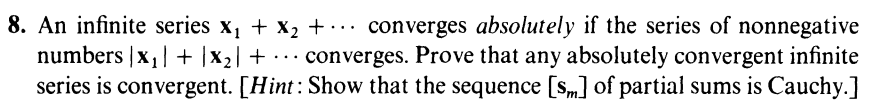
\includegraphics[width=1\textwidth]{MA-2-23-8.png}
\end{figure}
\end{question}
\begin{solution}
Fix $\epsilon > 0$. As the series converges absolutely, we have that
$\{ a_n = \sum_{i=1}^{n} |x_i| \}$ converges, hence is Cauchy.
As $\{a_n \}$ is Cauchy, 
there exists an index $N$ such that
\eQb
\sum_{i=n}^{m} |x_i| &=& |a_m - a_n| \\
&<& \epsilon,
\eQe
for $m \geq n \geq N$. 
Observe that for $m \geq n \geq N$, by the triangle inequality and 
the above inequality, we have
\eQb
|\sum_{i=1}^{m} x_i - \sum_{i=1}^{n} x_i| &=& |\sum_{i=n}^{m} x_i| \\
&\leq& \sum_{i=m}^{n} |x_i| < \epsilon. 
\eQe
Since $\epsilon > 0$ was arbitrary, 
this shows that $\{ \sum_{i=1}^{n} x_i \}$ is Cauchy. Since the sequence is 
drawn from a Euclidean space, we have shown that it is convergent.

\hfill $\qed$
\end{solution}

\newpage

\begin{question}[2]
\hfill
\begin{figure}[h!]
  \centering
    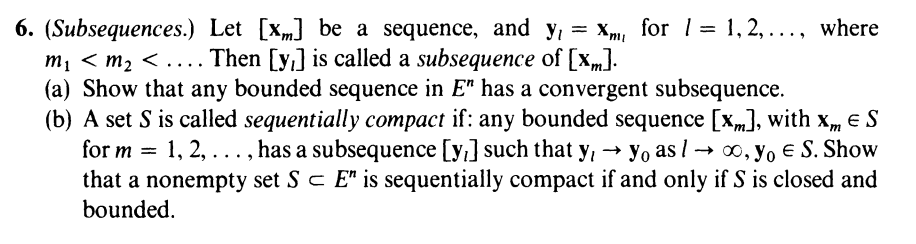
\includegraphics[width=1\textwidth]{MA-2-24-6.png}
\end{figure}
\end{question}
\begin{solution}
Correction: Drop the boundedness assumption from sequentially compact definition.
\textbf{(a)}
Let $\{ x^k \}$ be a bounded sequence in $E^n$. It follows that the sequences formed
by each component are bounded as well, as otherwise it would contradict the boundedness
of the original sequence in $E^n$. Now, consider the sequence of reals 
from the first component $\{x^k_{1}\}$. By Bolzano-Weiestrass theorem, we have that
there exists a convergent subsequence $\{x^{k_i}_{1}\}$. Now, consider the sequence of
reals from the second component $\{x^k_{2}\}$ and form a subsequence using the
subsequence indices from the convergent subsequence from the first component, which 
we denote as $\{ x^{k_i}_{2}\}$. Now, by Bolzano-Weiestrass theorem, once again,
we get a convergent subsequence of the second component sequence, with a property
that it is also a subsequence of the convergent subsequence from the first component sequence.
We do the above construction inductively until we get a convergent subsequence for the
$n$th component's convergent subsequence, whose indices we denote as $k_l$.
By construction, it follows that $\{x^{k_l}_i\}$ is a convergent sequence for $i = 1,2..,n$,
and they are subsequences of $\{x^k_i\}$ respectively. By preposition $2.7$, pg.$38$, we have
the sequence $\{ x^k_l\}$ converges, as each of its component sequence converges. Hence, we have
constructed a convergent subsequence of $\{x^k\}$. Therefore, we have shown that 
a bounded sequence in $E^n$ has a convergent subsequence. \\ 
\hfill $\qed$
 
\bigskip

\textbf{(b)} Assume that $S$ is closed and bounded.
Let $\{ x_m \}$ be a bounded sequence from $S$. Since $S$ is bounded, by $(a)$, there exists
a convergent subsequence $\{x_{m_k} \}$. Now, observe that $\{ x_{m_k}\}$ is a sequence in $S$,
and by the closedness of $S$, we have that the limit of $\{x_{m_k}\}$ is in $S$. Hence, we have
shown that there exists a convergent subsequence that converges to a point in $S$. $S$ is sequentially
compact. 

\smallskip

Assume that $S$ is sequentially compact. Let $\{ x_m \}$ be a sequence from $S$ such that $x_m \to
x$ as $m \to \infty$. Fix $\epsilon > 0$. Then, there exists an $N$ such that $|x_m - x| < \epsilon$
for $m \geq N$. Consider $\{x_m \}_{m \geq N}$. This is a bounded sequence in $S$, and it is also
a subsequence of $\{x_m\}$, whose limit is $x$, as any subsequence of a convergent sequence 
converges to the limit of the original sequence. By the sequential compactness assumption, we have that
$x \in S$. Since the sequence that was considered was arbitrary, we have shown that $S$ is closed. Now,
suppose for sake of contradiction that $S$ is not bounded. Then, there exists a sequence $\{x_m \}$
such that $|x_m| \geq m$. Observe that every subsequence of this sequence is not Cauchy, hence
not convergent. Therefore, it is a contradiction to the sequential compactness. Hence, $S$
is bounded.

\hfill $\qed$
 

\end{solution}

\newpage

\begin{question}[3]
\hfill
\begin{figure}[h!]
  \centering
    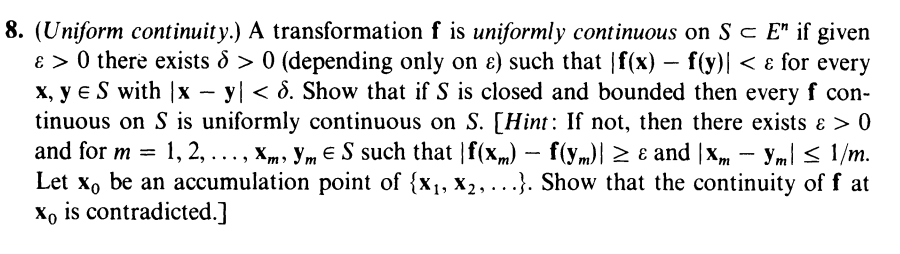
\includegraphics[width=1\textwidth]{MA-2-25-8.png}
\end{figure}
\end{question}
\begin{solution}
Let $S$ be a closed and bounded set in $\mathbb{R}^n$ and $f$ be a continuous transformation. 
on $S$.
We know that a closed bounded set in $\mathbb{R}^n$ is compact. Therefore, we prove the following
more general theorem.

\smallskip

\begin{theorem}
\textit{ 
Let $f:X \to Y$, such that $f$ is continuous, $X,Y$ are metric spaces, and $X$ is compact. 
Then, $f$ is uniformly continuous.} 
\end{theorem}
\begin{proof}
Fix $\epsilon > 0$. As $f$ is continuous on $X$, for any $x \in X$, there exists $\delta_x > 0$
that corresponds to the $\frac{\epsilon}{2}$-challenge. Then, we have
\eQb
X &=& \bigcup_{x \in X} B(x,\delta_x).
\eQe
Now, observe that the sets in the RHS form an open cover of $X$. Since $X$ is compact,
the open cover has a finite sub-cover. Thus, we can write $X$ as follows: 
\eQb
X &=& \bigcup_{i=1}^{n} B(x_i, \delta_{x_i}),
\eQe
where $x_i$ are from $X$ and $\delta_{x_i}$ are the values that correspond to the 
$\frac{\epsilon}{2}$ challenge at $x_i$.
Now, let $\delta = \dfrac{\min_{i = 1,2..,n}(\delta_{x_i})}{2}$.
We claim that $\delta$ corresponds to the $\epsilon$-challenge of uniform continuity. 
Let $x,y \in X$, such that $d(x,y) < \delta$. It follows that there exists $x_i \in X$,
such that $x,y \in B(x_i, \delta_{x_i})$.
By the triangle inequality, and the continuity of $f$ at $x_i$,
we have
\eQb
|f(x) - f(y)| &=& |f(x) - f(x_i) + f(x_i) - f(y)| \\
&\leq& |f(x) - f(x_i)| + |f(x_i) - f(y)| \\
&<& \dfrac{\epsilon}{2} + \dfrac{\epsilon}{2} = \epsilon.
\eQe
Hence, $\delta$ corresponds to the $\epsilon$-challenge of uniform continuity of $f$.
Since $\epsilon > 0$ was arbitrary, we have shown that $f$ is uniformly continuous. 
\end{proof}
As a corollary, it follows that if $S$ is closed and bounded, then every continuous function
$f$ is uniformly continuous on $S$. 
\hfill $\qed$

\end{solution}

\newpage

\begin{question}[4]
\hfill
\begin{figure}[h!]
  \centering
    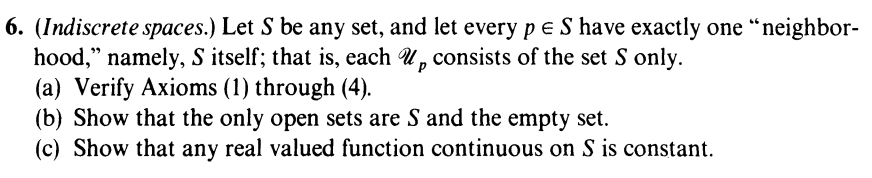
\includegraphics[width=1\textwidth]{MA-2-26-6.png}
\end{figure}
\end{question}
\begin{solution}
\textbf{(a)} For any point $p \in S$, and we have defined
$S$ as a neighborhood of $p$. Hence, there is a neighborhood of $p$.  
The axiom $(1)$ is satisfied.

\smallskip 
Let $p \in S$. We have that the only neighborhood of $p$ is $S$. Since $p \in S$, the
axiom $(2)$ is satisfied.

\smallskip

Let $p \in S$, $U_1$ and $U_2$ be neighborhoods of $p$.
Since $S$ is the only neighborhood of $p$, we have $U_1 = U_2 = U_1 \cap U_2 = S$. 
Since $S \subset S$, the axiom $(3)$ is satisfied. 

\smallskip

Let $p \in S$, $U$ be a neighborhood of $p$, and $q \in U$. We have $U =S$ and $S$
is a neighborhood of $q$ by definition. Since $S \subset S$, the axiom $(4)$ is satisfied. 

\bigskip

\textbf{(b)}
By the 4th axiom, we have that any neighborhood is an open set. Hence, $S$ is open. 
$\emptyset$ is open, because the statement of open holds vacuously. Now, let $A$ be 
a nonempty subset of $S$ such that $A \neq S$. Since $A$ is nonempty, there exists
a point $p \in A$, and by definition of the topology, $p$ has $S$ as a neighborhood. 
Since $A \neq S$, $S \not\subset A$, and we have that $p$ is not interior to $A$.
Hence, $A$ is not open. We have shown that $S$ and $\emptyset$ are the only open sets.

\bigskip

\textbf{(c)} Let $f:S \to \mathbb{R}$ be continuous with respect to the indiscrete topology.
By the corollary $2.6.2$ in Fleming, pg.$53$, we have that $\{p : f(p) > c \}$ is open
for any $c \in \mathbb{R}$. Assume that $f$ is not a constant function. Then, it follows
that there exists $p_1 \neq p_2 \in S$ such that $f(p_1) \neq f(p_2)$. Since $f(p_1) 
\neq f(p_2)$, we have either $f(p_1) > f(p_2)$ or $f(p_1) < f(p_2)$. As the cases are
symmetric, assume without loss of generality that $f(p_1) > f(p_2)$. It follows that 
$f(p_1) > \dfrac{f(p_1) + f(p_2)}{2} > f(p_2)$. Now, consider $A = \{ p : f(p) > 
\dfrac{f(p_1) + f(p_2)}{2} \}$. We have that $p_1 \in A$ and $p_2 \not\in A$. Therefore,
we have that $A$ is nonempty and $A \neq S$. By the corollary, we have that $A$ is open, but
we have previously shown that $S$ and $\emptyset$ are the only open sets. Hence, we have
reached a contradiction and $f$ must be a constant function.

\hfill $\qed$
 
\end{solution}

\newpage

\begin{question}[5]
\hfill
\begin{figure}[h!]
  \centering
    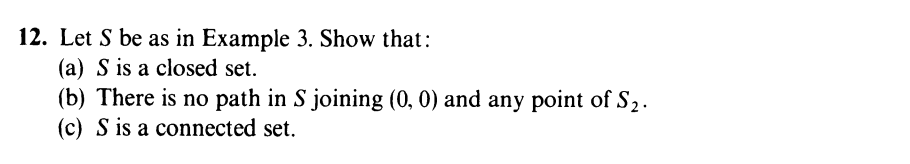
\includegraphics[width=1\textwidth]{MA-2-27-12.png}
\end{figure}
\end{question}
\begin{solution} 
 
 
\end{solution}

\newpage

\begin{question}[6]
\hfill
\begin{figure}[h!]
  \centering
    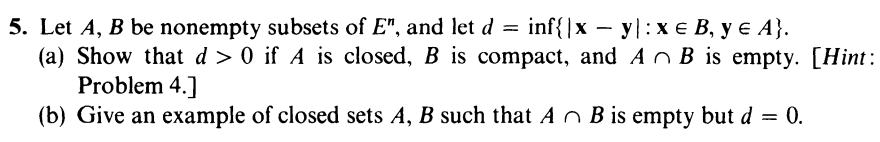
\includegraphics[width=1\textwidth]{MA-2-28-5.png}
\end{figure}
\end{question}
\begin{solution} \hfill \\ 
\textbf{(a)} Suppose for sake of contradiction that $d(A,B) = 0$. As $d(A,B) = 0$, we can choose
a sequence of $\{(a_n,b_n)\}_{n=1}^{\infty}$ such that $\lim_{n \to \infty} |a_n - b_n| = 0$,
by using the approximation property of infimum.  
As $B$ is compact, there exists a subsequence $\{b_{n_k} \}$ such that it converges to some $b$ 
in $B$. We claim that the corresponding subsequence $\{a_{n_k} \}$ converges to $b$. Fix $\epsilon > 0$.
Then, there exists $K_1$ such that $|b - b_{n_k}| < \dfrac{\epsilon}{2}$ for $k \geq K_1$. Furthermore, 
there exists $K_2$ such that $|a_{n_k} - b_{n_k}| < \dfrac{\epsilon}{2}$ for $k \geq K_2$. 
Let $K = \max(K_1, K_2)$.
It follows that 
\eQb
|a_{n_k} - b| &=& |a_{n_k} - b_{n_k} + b_{n_k} - b| \\
&\leq& |a_{n_k} - b_{n_k}| + |b_{n_k} - b| < \epsilon,
\eQe
for $k \geq K$. Hence, we have shown that $a_n \to b$ as $n \to \infty$. Since $A$ is closed, 
we have that $b \in A$ and this is a contradiction with $A \cap B = \emptyset$. Therefore,
we have that $d(A,B) = 0$. 

\bigskip

\textbf{(b)}
Let $A = \mathbb{N}$ and $B = \{ n + \dfrac{1}{n} \> | \> n \in \mathbb{N} \}$. Observe that
both sets are closed, and $A \cap B = \emptyset$, but $d(A,B) = 0$, as for any $\epsilon > 0$,
by Archemedian property of the real, there is a large enough $n$, where $\dfrac{1}{n} < \epsilon$.

\hfill $\qed$
 
\end{solution}
\newpage

\begin{question}[7]
\hfill
\begin{figure}[h!]
  \centering
    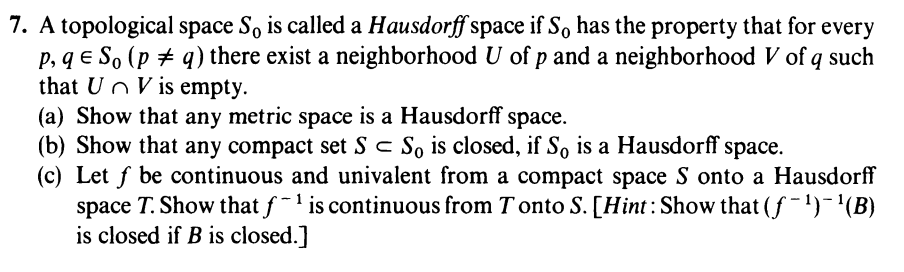
\includegraphics[width=1\textwidth]{MA-2-29-7.png}
\end{figure}
\end{question}
\begin{solution} 
\textbf{(a)}
Let $(X,d)$ be a metric space, with $p_1 \neq p_2 \in X$. By one of the axioms of 
metric spaces, we have that $d(p_1, p_2) > 0$. Let $\delta = \dfrac{d(p_1, p_2)}{2}$,
and consider $B_1 = B(p_1,\delta)$ and $B_2 = B(p_2,\delta)$. We claim that $B_1 \cap
B_2 =\emptyset$. Suppose that there exists $p \in X$ such that $p \in B_1 \cap B_2$.
It follows that $d(p,p_1) < \delta$ and $d(p,p_2) < \delta$. By the triangle inequality,
we have
\eQb
d(p_1, p_2) &\leq& d(p_1,p) + d(p,p_2) \\
&<& \delta + \delta = d(p_1, p_2).
\eQe  
Hence, we have shown that $d(p_1, p_2) < d(p_1, p_2)$, which is a contradiction. 
Therefore, $B_1 \cap B_2 = \emptyset$. Since $p_1$ and $p_2$ were arbitrary two
distinct points from $X$, we have shown that a metric space is Hausdorff. 
\hfill $\qed$

\bigskip

\textbf{(b)}
Let $S_0$ be a Hausdorff space, and $S$ be a compact subset of $S_0$.
Let $x \in S_0 \setminus S$. Now, for any $s \in S$, by Hausdorff property 
of $S_0$, there exists a neighborhood of $x$, $N_x$, and a neighborhood of $s$, $N_s$,
such that $N_x \cap N_s = \emptyset$. Observe that 
\eQb
S \subset \bigcup_{s \in S} N_s.
\eQe  
As the RHS is an open cover of $S$, by compactness of $S$, there exists a finite
sub-cover $\{N_{s_i}\}_{i=1}^{n}$ such that 
\eQb
S \subset \bigcup_{i=1}^{n} N_{s_i},
\eQe
with the corresponding neighborhood of $x$, selected via Hausdorff property
denoted as $\{ N_{x_i} \}_{i=1}^{n}$. As an intersection of finite collection
of open sets is open, we have that $\bigcap_{i=1}^{n} N_{x_i}$ is open. Furthermore,
it is a neighborhood of $x$, that is disjoint from $\bigcup_{i=1}^{n} N_{s_i}$,
thus from $S$ as well. Since $x$ was chosen arbitrarily from $S_0 \setminus S$, we have
shown that $S_0 \setminus S$ is open. Hence, $S$ is closed.
\hfill $\qed$

\bigskip

\textbf{(c)} We first prove a simple central lemma:
\begin{lemma}[7.c. Closedness implies Compactness in Compact Space]
\textit{Let $X$ be a compact topological space, and $A$ be a closed subset of $X$.
Then, $A$ is compact}.
\end{lemma}
\begin{proof}
Let $\{O_{\lambda}\}$ be an open cover of $A$. As $A$ is closed, $X\setminus A$ is open,
and we have that $\{O_{\lambda}\}$ with $X \setminus A$ is an open cover of $X$. By
compactness of $X$, there exists a finite subcover of the open cover that covers $X$. 
Remove $X \setminus A$ if its in the finite subcover. Since we only removed $X \setminus
A$, the finite subcover still covers $A$. Also, it is a finite 
subcover of the original open cover of $A$. Hence, we have shown that $A$ is compact. 
\end{proof}

We wish to show that $f^{-1}$ is continuous. We know that 
a function is continuous iff an inverse image of a closed set is closed.
Hence, it suffices to show that for a closed subset $B$ of $S$,
 $(f^{-1})^{-1}(B)$ is closed. Note that $(f^{-1})^{-1}(B) = f(B)$.
Let $B$ be a closed subset of $S$. By the established lemma, 
as $B$ is closed, $B$ is compact. By the theorem $2.10$ on pg.$61$ in Fleming,
since $f$ is continuous, $f(B)$ compact. We have shown that a compact subset is
closed in Hausdroff space in part $(b)$. Therefore, $f(B)$ is closed.
We have shown that $f^{-1}$ is continuous. 
\hfill $\qed$


\end{solution}
\newpage

\begin{question}[8]
\hfill
\begin{figure}[h!]
  \centering
    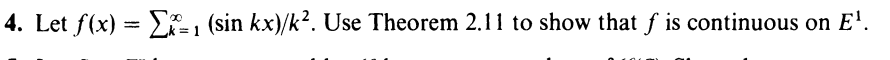
\includegraphics[width=1\textwidth]{MA-2-210-4.png}
\end{figure}
\end{question}
\begin{solution} 
To begin with, we note that the function is well-defined as
for a fixed $x \in \mathbb{R}$, $\sum_{k=1}^{\infty} \dfrac{\sin(kx)}{k^2}$
converges absolutely. 
The absolute convergence of the series can be shown through a comparison
test with $\sum_{k=1}^{\infty} \dfrac{1}{k^2}$. 
Now, we denote the $n$th partial sum function as $f_n$. Observe that $\{ f_n \}$ 
forms a sequence of continuous functions, as $\sin(kx)/k^2$ is continuous 
for all $k \in \mathbb{N}$ and a sum of two continuous function is continuous.
Furthermore, observe that $f_n \in \mathbb{B}(E)$ for all $n$, as $|\sum_{k=1}^{n} 
\dfrac{\sin(kx)}{k^2}| \leq \sum_{k=1}^{n} \dfrac{1}{k^2} <\infty$ for all 
$x \in E$. Since $B(E)$ forms a complete metric space with respect to the supnorm,
showing that $\{f_n \}$ is Cauchy in supnorm will give us that $\{ f_n \}$ convergent
in supnorm, which then gives uniform convergence of $\{f_n\}$.

\bigskip

Fix $\epsilon > 0$. Now, since $\sum_{k=1}^{\infty}\dfrac{1}{k^2}$ is convergnt, 
there exists an index $N$ such that for all $n \geq m \geq N$, we have
$\sum_{k=m}^{n} \dfrac{1}{k^2} < \epsilon$. Observe that, for $n \geq m \geq N$,
\eQb
|f_n - f_m | &=& \left| \sum_{k=1}^{n} \dfrac{\sin(kx)}{k^2} - 
\sum_{k=1}^{m} \dfrac{\sin(kx)}{k^2} \right| \\
&=& \left| \sum_{k=m}^{n} \dfrac{\sin(k)}{k^2} \right| \\
&\leq& \sum_{k=m}^{n} \left| \dfrac{\sin(k)}{k^2} \right| \\
&\leq& \sum_{k=m}^{n} \dfrac{1}{k^2} < \epsilon. \\ 
\eQe 
Since $\epsilon > 0$ was arbitrary, we have shown that $\{f_n \}$ is Cauchy in $\mathbb{B}(E)$,
with respect to the supnorm, hence $\sum_{k=1}^{\infty}\dfrac{\sin(kx)}{x^2}$ is a uniform limit
of a series of continuous function on $E$.
 By Theorem 2.11, we have that $f$ is continuous on $E$
 as required.
\hfill $\qed$
\end{solution}

\newpage

\begin{question}[9]
\hfill
\begin{figure}[h!]
  \centering
    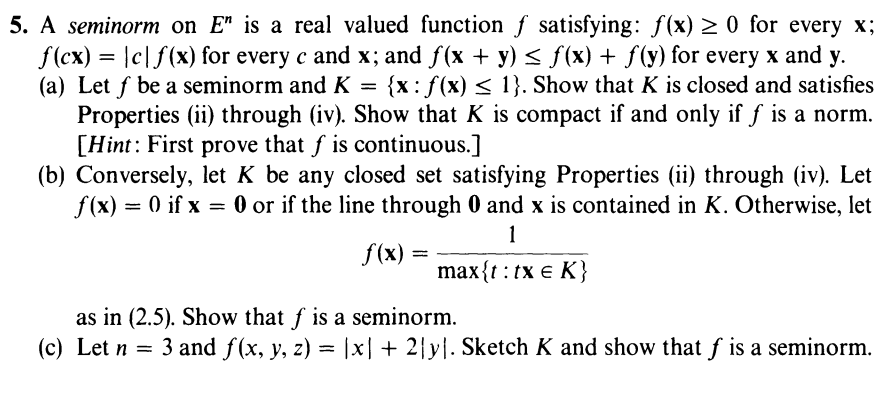
\includegraphics[width=1\textwidth]{MA-2-211-5.png}
\end{figure}
\end{question}
\begin{solution} 
\textbf{(a)}

\bigskip

\textbf{(b)}

\bigskip

\textbf{(c)}
We first show that $f(x,y,z)$ is a semi-norm. Let $(x,y,z) \in E^3$, and $c \in E$. It follows that
$0 \leq |x| + 2|y| = f(x,y,z)$ and $f(cx,cy,cz) = |cx| + 2|cy| = |c||x| + 2|c||y| = |c|f(x,y,z)$. 
Now, let $a = (x_1,y_1,z_1)$ and $b = (x_2, y_2, z_2)$ in $E^3$. It follows that 
\eQb
f(a+b) &=& |x_1 + x_2| + 2|y_1 + y_2| \\
&\leq& |x_1| + |x_2| + 2|y_1| + 2|y_2| = f(a) + f(b). 
\eQe 
Therefore, we have shown that $f$ is a semi-norm.
We plot the figure below. 
\begin{figure} [h!]
\centering
\begin{subfigure}{.5\textwidth}
  \centering
  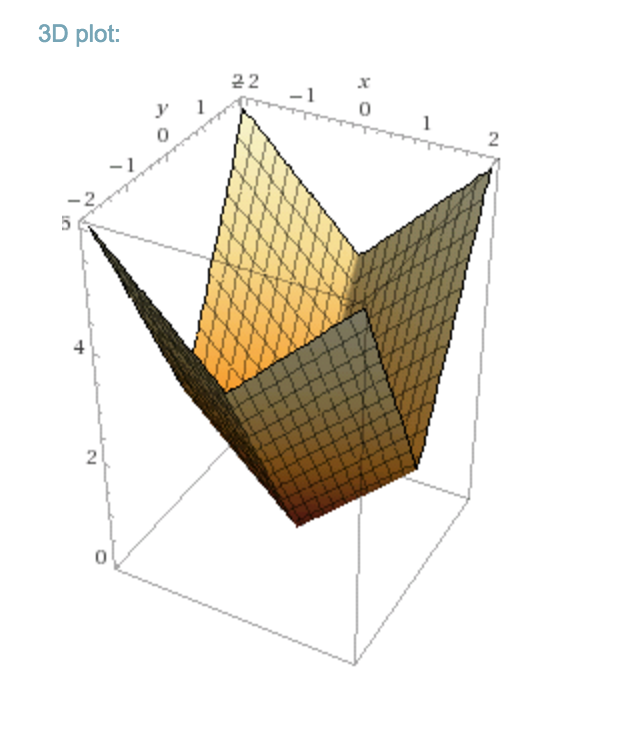
\includegraphics[width=.6\linewidth]{multi-plot1}
  \caption{3D-figure}
  \label{fig:sub1}
\end{subfigure}%
\begin{subfigure}{.5\textwidth}
  \centering
  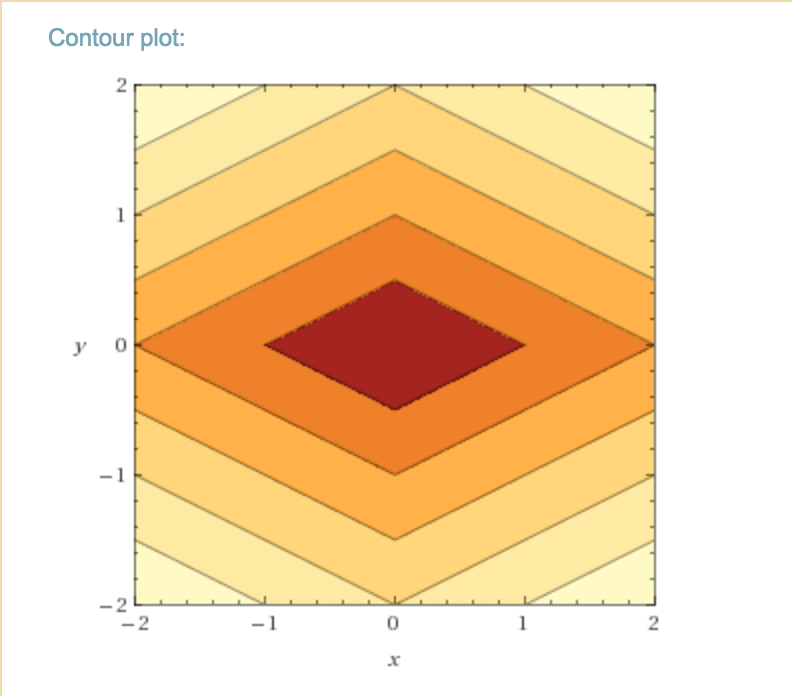
\includegraphics[width=.6\linewidth]{multi-plot2}
  \caption{Contours}
  \label{fig:sub2}
\end{subfigure}
\caption{Plot of $f(x,y,z) = |x| + 2|y|$}
\label{fig:test}
\end{figure}
\hfill \\
\hfill $\qed$ 
 
\end{solution}

\newpage

\end{document}
